% This is samplepaper.tex, a sample chapter demonstrating the
% LLNCS macro package for Springer Computer Science proceedings;
% Version 2.20 of 2017/10/04
%
\documentclass[runningheads]{llncs}
%

\usepackage{graphicx}
\graphicspath{ {\string~/Documents/retele_tema2/retele_pics} }

% Used for displaying a sample figure. If possible, figure files should
% be included in EPS format.
%
% If you use the hyperref package, please uncomment the following line
% to display URLs in blue roman font according to Springer's eBook style:
% \renewcommand\UrlFont{\color{blue}\rmfamily}

\begin{document}
%/Users/teodorciripescu
\title{Offline Messenger (B)}
%
%\titlerunning{Abbreviated paper title}•
% If the paper title is too long for the running head, you can set
% an abbreviated paper title here
%
\author{Ciripescu Teodor\\
\email{teodor.ciripescu@info.uaic.ro}\\}
%
% First names are abbreviated in the running head.
% If there are more than two authors, 'et al.' is used.
%
\institute{Facultatea de Informatica, UAIC\\
}
%
\maketitle              % typeset the header of the contribution
%
\begin{abstract}
Acest document contine planul de implementare pentru proiectul "Offline Messenger".

\end{abstract}
%
%
%
\section{Introducere}
%Indicatii pentru rezolvarea Temei 2 (care va contine si portiuni de cod)
%Structura generala pe sectiuni a raportului va fi urmatoarea:
%- Introducere
%- Tehnologiile utilizate (e.g. TCP, UDP... - caracteristicile care au fost utilizate in cadrul proiectului). Justificati de ce ati ales aceste tehnologii.
%- Arhitectura aplicatiei (conceptele implicate, diagrama aplicatiei detaliata)
%- Detalii de implementare (cod relevant particular proiectului, care va fi documentat; scenarii de utilizare)
%- Concluzii (e.g. cum ar putea fi imbunatatita solutia propusa?)
%- Bibliografie
%Termen de predare: laboratorul din saptamana 11.

%Sa se dezvolte o aplicatie client/server care sa permita schimbul de mesaje intre utilizatori care sunt conectati si sa ofere functionalitatea trimiterii mesajelor si catre utilizatorii offline, acestora din urma aparandu-le mesajele atunci cand se vor conecta la server. De asemenea, utilizatorii vor avea posibilitatea de a trimite un raspuns (reply) in mod specific la anumite mesaje primite. Aplicatia va oferi si istoricul conversatiilor pentru si cu fiecare utilizator in parte.
Aceasta abordare a proiectului Offline Messenger va avea in prim plan dezvoltarea unor sisteme de: autentificare/inregistrare a utilizatorilor, "prietenie" intre utilizatori,  stocare/procesare a conversatiilor dintre utilizatori, notificari din partea serverului in legatura cu anumite evenimente. Vom utiliza un server TCP concurent cu threaduri. Pentru fiecare client va fi folosit un thread ce va fi eliminat odata cu deconectarea clientului de la server.\\
Pentru stocarea datelor va fi folosita o baza de date sqlite.\\
Pentru facilitarea de dezvoltare a unui client web, va fi prezenta si o abordare a raspunsurilor de tip JSON din partea serverului.\\
\section{Autentificarea/Inregistrarea utilizatorilor}
La inregistrare clientul isi alege un username (unic) si o parola. Acestea vor fi stocate in baza de date sub tabela users (parola va fi hash-uita). \\
La autentificare se va cere ca input un username si o parola, daca username-ul exista si daca hash-ul parolei date ca input coincide cu cel prezent in baza de date, clientul este autentificat. Acum are acces la o serie de comenzi specifice utilizatorilor. \\
%De fiecare data cand cand un utilizator apeleaza o comanda catre server, acesta va servi si ID-ul unic specific, pentru ca serverul sa stie cine i se adreseaza.\\
In cazul unor impedimente precum: cineva incearca sa se inregistreze cu un username deja existent, parola scrisa la autentificare este gresita etc ..., clientul va fi atentionat de catre server.\\

\section{Sistem de "Prietenie" intre utilizatori}
Fiecare utilizator autentificat va putea trimite cereri de prietenie catre alti utilizatori. In cazul in care aceste cereri sunt acceptate, vor putea incepe conversatii intre utilizatorii respectivi. \\
Cand un client se autentifica vor fi cerute de la server si salvate in memorie listele de prieteni, conversatiile si cererile de prietenie. Aceste liste vor fi modificate pe parcursul rularii in functie de evenimentele petrecute. Stocarea informatiilor este vitala pentru a evita comunicarea nenecesara cu serverul.\\
Utilizatorii vor putea sa isi vada lista de prieteni, sa trimita cereri de prietenie, sa isi vada lista cererilor de prietenie primite si sa accepte sau sa refuze cererile de prietenie.\\

\section{ Procesarea/Stocarea Conversatiilor }
Un client autentificat poate trimite altor clienti din lista sa de prieteni mesaje. Aceste mesaje vor avea asociate in baza de date campuri precum time, seen si reply\_to pentru a determina cand a fost trimis un mesaj, daca a fost vazut destinatar si daca reprezinta o replica la alt mesaj. Mesajele vor avea optiunea de a fi sterse (atat pentru o singura persoana cat si pentru ambele).\\
\section{Notificari}
Utilizatorii vor fi notificati de catre server cand au loc anumite evenimente: mesaj nou primit, cerere noua de prietenie. De asemenea, in momentul autentificarii, clientii vor fi atentionati de mesajele si cererile de prietenie pe care le-au primit pe perioada in care au fost offline.\\
\section{Protocol}
Fiecare client va avea asociat threadul lui pe server si o structura in care va fi memorat descriptorul si ID-ul de utilizator obtinut la autentificare. Threadul va inceta sa mai existe in momentul in care clientul se deconecteaza de la server.\\ 
Mai intai se vor trimite 2 bytes pentru a semnala lungimea comenzii.\\
Apoi va fi trimisa comanda propriu-zisa, formata din 1 byte pentru codul comenzii (comenzile vor fi indexate printr-un numar), iar restul de bytes vor fi folositi pentru lungimea parametrilor si parametri.\\
Raspunsul primit de client va fi format asemanator, 2 bytes pentru lungimea raspunsului, 1 byte pentru comanda folosita, iar restul pentru mesajul propriu-zis.\\
Va fi folosit un thread nou in care clientul asteapta mesaje noi de la server. Astfel va fi evitat un blocaj in care incercam sa scriem si se citim in acelasi timp.\\
Am ales folosirea threadurilor pentru ca sunt mai eficiente, mai lightweight decat o abordare cu procese copil. Mai mult, natura proiectului implica prezenta multor clienti conectati la server in acelasi timp, cat si citiri/scrieri  constante la server. Taskurile date serverului sunt in general simple si multe, deci se preteaza mai bine pe modelul cu threaduri.\\
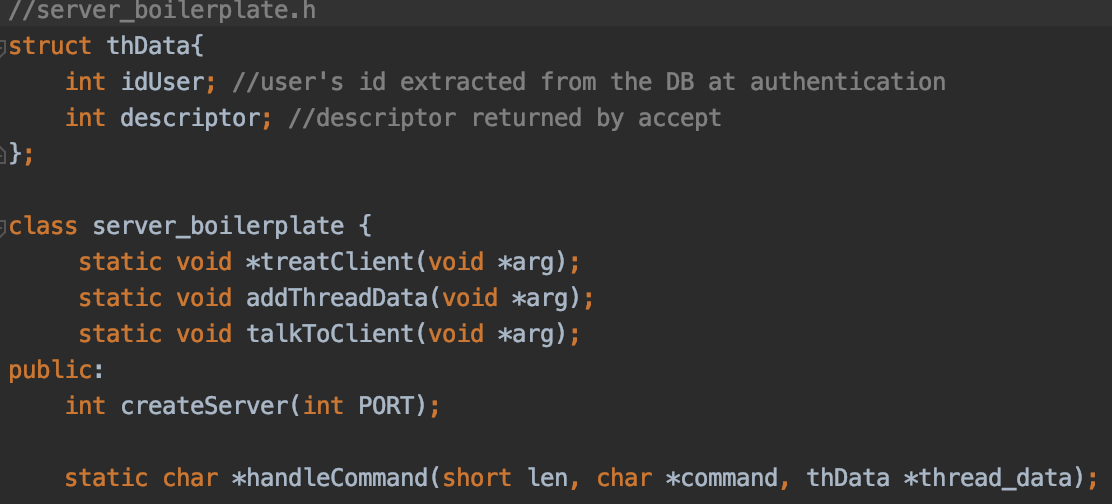
\includegraphics[width=100mm,scale=1]{retele_pics/boilerplate_header.png}\\
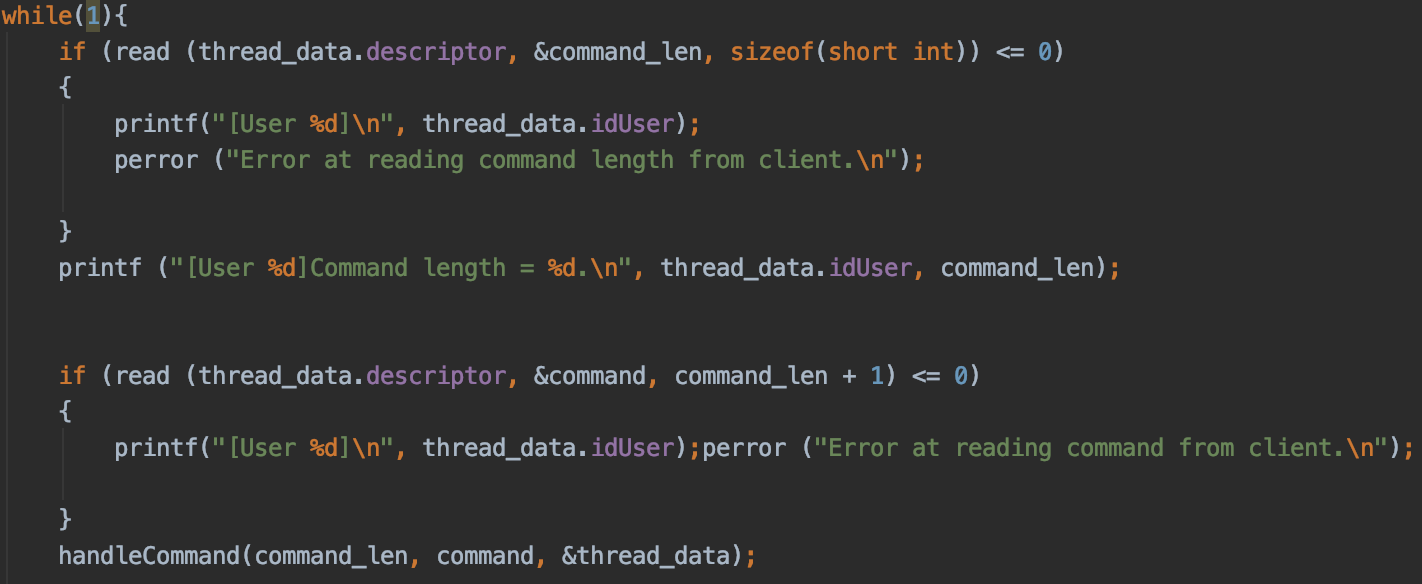
\includegraphics[width=100mm,scale=1]{retele_pics/reading_handling_cmd.png}\\

\subsubsection{Comenzi si evenimente ce au loc in urma executarii lor de catre utilizatori}\hfill\\

Fiecare client ce se conecteaza la server poate folosi una dintre urmatoarele comenzi:\\
-register(username, password) $\rightarrow$ Daca a avut succes sau nu;\\
-authenticate(username, password) $\rightarrow$ daca are loc cu succes, clientul capata titlul de utilizator si va avea drepturi extra\\

Fiecare utilizator va putea folosi urmatoarele comenzi:\\
getFriendList() $\rightarrow$ Lista cu ID-urile prietenilor;\\
sendFriendRequest(username) $\rightarrow$ cererea (nu) a fost trimisa;\\
getFriendRequestList() $\rightarrow$ Lista cu ID-urile cererilor care nu au fost solutionate;\\
acceptFriendRequest(request\_id);\\
rejectFriendRequest(request\_id);\\
getConversations() $\rightarrow$ Lista cu ID-urile conversatiilor;\\
getMessages(id\_conversation, messages\_amount) $\rightarrow$ ultimele  *messages\_amount* din conversatia *id\_conversation*;\\
getAllMessages(params: id\_coversation) $\rightarrow$toate mesajele din converastia
*id\_conversation*;\\
sendMessage(id\_conversation, content) $\rightarrow$ mesajul (nu) a fost trimis;\\
replyMessage(id\_conversation, id\_message\_toReply, content) $\rightarrow$ mesajul (nu) a fost trimis;\\
deleteMessage(id\_message, for\_me/for\_all ) $\rightarrow$ mesajul (nu) a fost sters;\\
logout();\\
Exemplu:
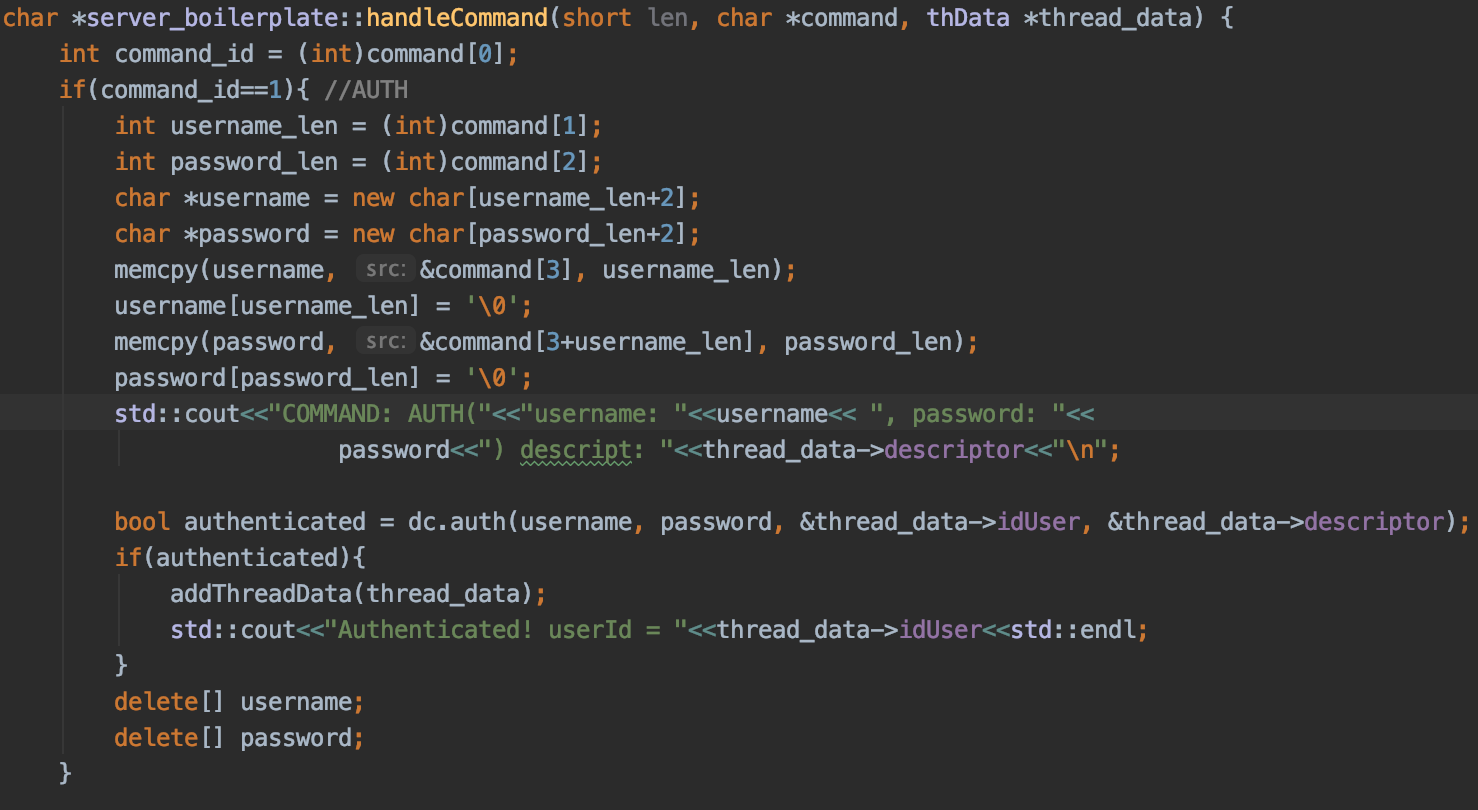
\includegraphics[width=130mm,scale=1]{retele_pics/auth_handle.png}\\

\subsubsection{Evenimente ce se petrec automat }\hfill\\
Serverul va notifica in momentul autentificarii pe utilizator in legatura cu: conversatii ce contin mesaje noi/necitite, noi cereri de prietenie.\\
Mesajele cu statutul de "necitit" vor avea statutul de "citit" daca acestea sunt continute in raspunsul intors de functiile "getMessages" sau "getAllMessages".\\
Utilizatorii vor fi notificati de noi cereri de prietenie si noi mesaje.\\
Daca 2 utilizatori nu sunt "prieteni" nu va fi posibila crearea unei conversatii intre cei 2.\\

\section{Baza de date}
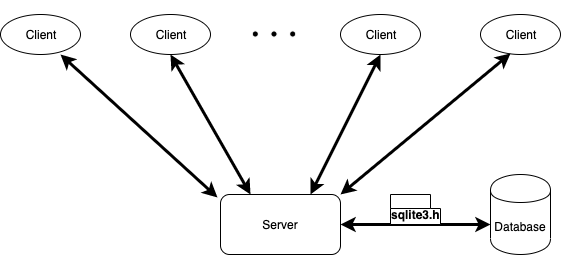
\includegraphics[width=100mm,scale=1]{retele_pics/general_diagram.png}\\
Vom folosi o baza de date sqlite pe care o vom accesa prin intermediul bibliotecii sqlite3.h . Toate apelurile catre baza de date vor fi facute de catre server in urma comenzilor date de catre clienti.\\
Baza de date va respecta urmatoarea schema:\\
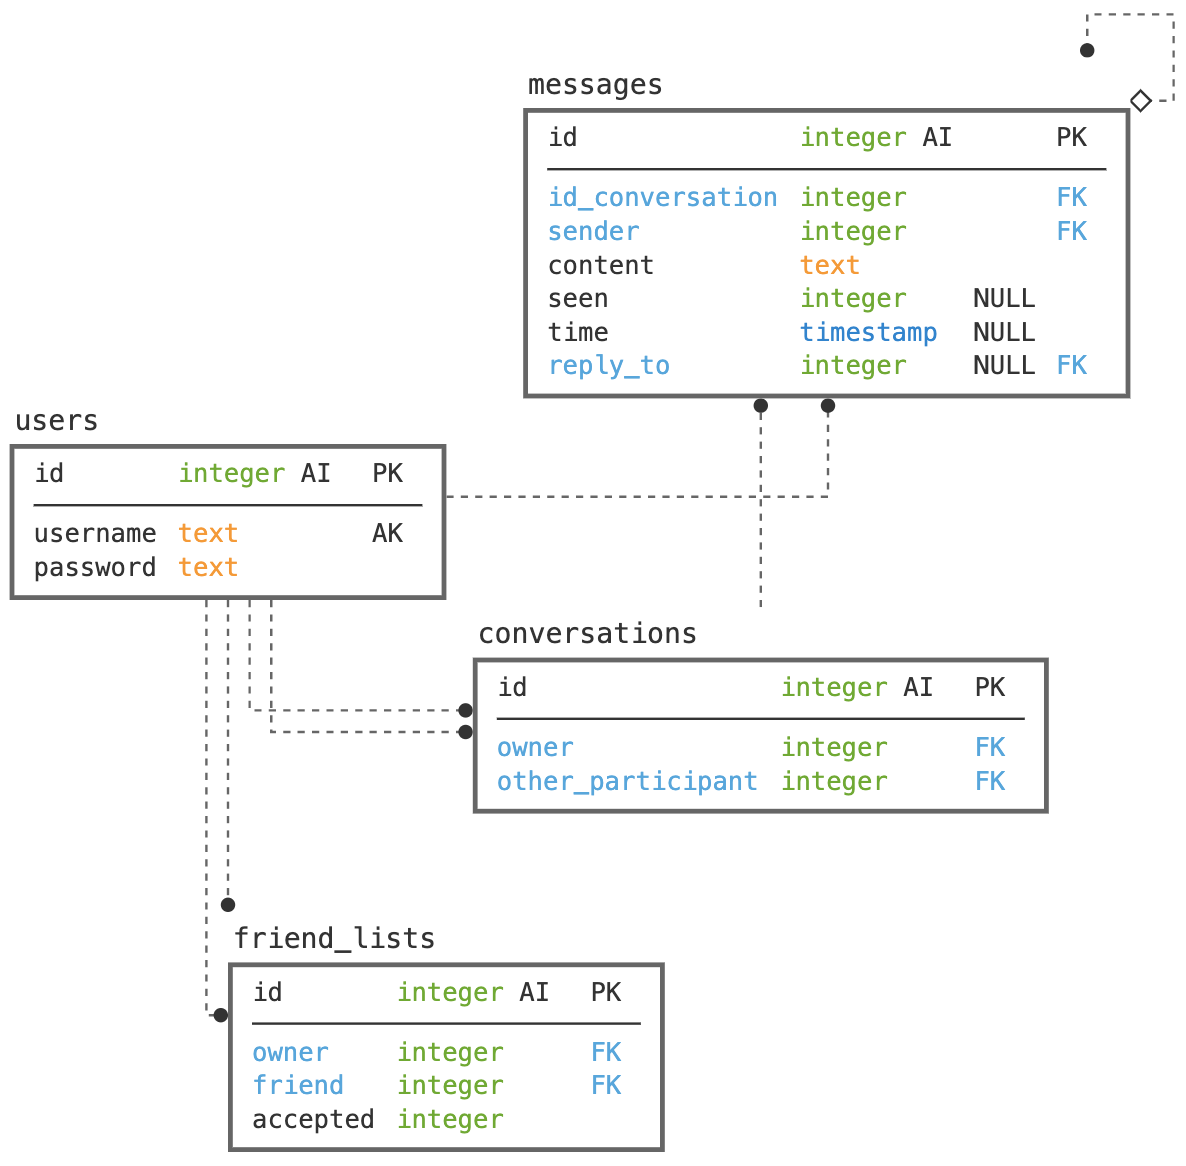
\includegraphics[width=100mm,scale=1]{retele_pics/database_schemas/diagram_light.png}\\
In lista de prieteni va fi inregistrata prietenia din ambele sensuri (poti sterge pe cineva ca prieten si el sa te aiba in continuare in lista);'\\
La fel si la conversatii, se poate pastra o conversatie cu cineva dar acel cineva sa nu o pastreze la randul sau.\\
Si mai mult, pe acelasi principiu se vor baza si mesajele, va fi o copie amesajului pentrut fiecare conversatie(respectiv utilizator) in parte. Astfel, va fi posibila stergerea mesajelor pentru fiecare client, fara sa fie nevoie sa se stearga mesajul si pt cealalta persoana. \\
Procedura de interogare a bazei de date pentru autentificare:\\
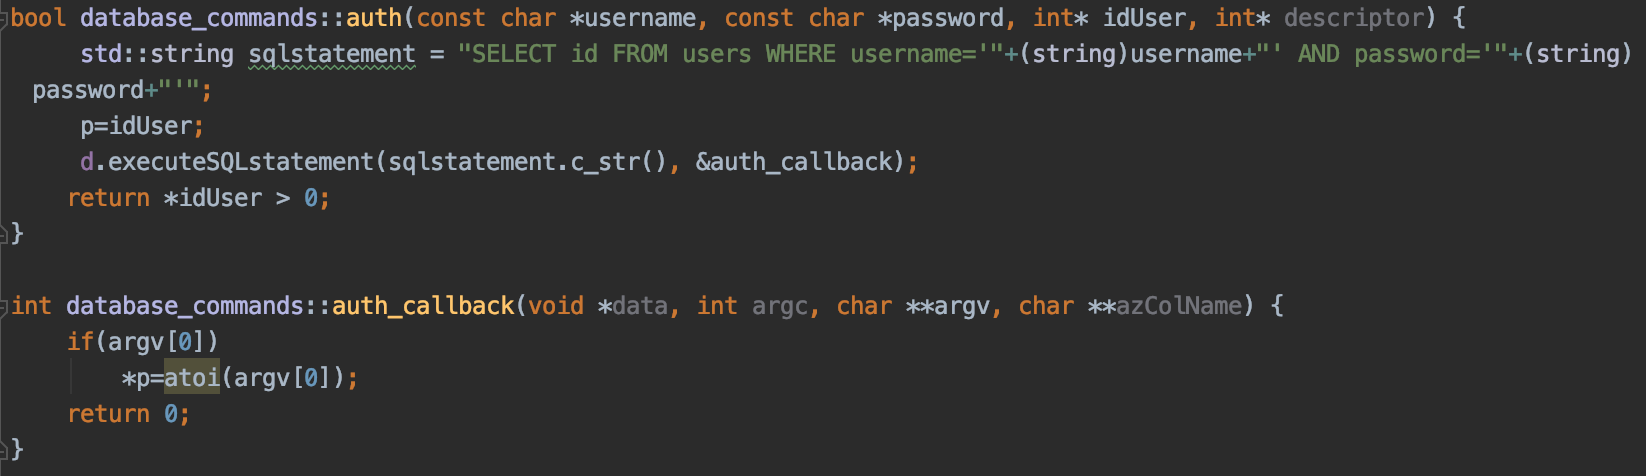
\includegraphics[width=145mm,scale=1]{retele_pics/db_query.png}\\
\section{Concluzii si posibile aditii}
Luand in considerare cele de mai sus putem intelege ca orice request al unui client catre server are urmatorulu drum. In prima instanta, clientul se conecteaza la server si un thread ii este alocat pentru managementul requesturilor. Detalii referitoare la client vor fi retinute intr-o structura de tipul thData (descriptorul si id-ul care initial este -1 din lipsa de autentificare). Acum singurele comenzi ce pot fi facute de catre client sunt register si authenticate. In urma unei autentificari cu succes (ce implica o interogare a bazei de date cu parametrii username si password), campului idUser din structura thData ii este atribuita valoarea id-ului asociat utilizatorului din tabela users a bazei de date. Clientul capata mai multe drepturi, si anume accesul la mai multe comenzi(prezentate mai sus). Proaspat autentificat, utilizatorul este notificat de ce a ratat in perioada in care a fost offline (mesaje noi, cereri de prieteni). Noi cereri de prietenie si mesaje noi vor aparea in continuare pe parcursul rularii.\\
In momentul in care un client doreste sa trimita un mesaj altui client, acesta va folosi una dintre functiile de trimitere mesaj catre server. Serverul va cauta in vectorul de structuri thData descriptorul destinatarului si ii va transmite mesajul prin acesta.\\
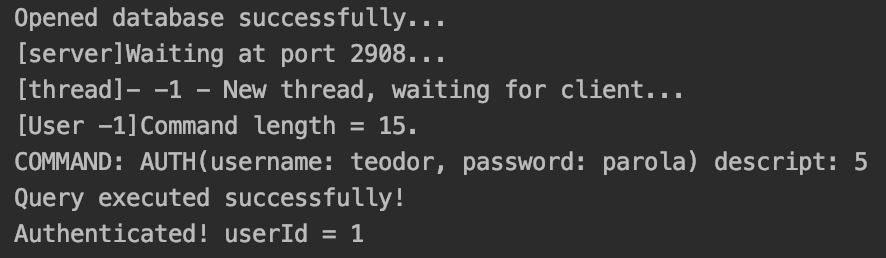
\includegraphics[width=100mm,scale=1]{retele_pics/auth_test.png}\\
Poate fi implementata si o solutie de criptare a mesajelor. Va trebui folosita o metoda de a securiza schimbul de chei ( Diffie Hellman key exchange).\\
\begin{thebibliography}{8}
\bibitem{ref_article1}
https://www.sqlite.org/whentouse.html
\bibitem{ref_article1}
https://www.sqlite.org/capi3ref.html
\bibitem{ref_article1}
https://profs.info.uaic.ro/~computernetworks/files/NetEx/S12/ServerConcThread/servTcpConcTh2.c
\bibitem{ref_article1}
https://profs.info.uaic.ro/~computernetworks/files/NetEx/S12/ServerConcThread/cliTcpNr.c
\bibitem{ref_article1}
https://www.geeksforgeeks.org/sql-using-c-c-and-sqlite/
\end{thebibliography}
\end{document}
